\lysh{12976}{2}

\begin{alist}
\item Επειδή $\alpha=2, \beta=-1$ και $\gamma=-1$ η διακρίνουσα είναι
$\Delta = (-1)^2 - 4 \cdot 2(-1) = 1 + 8 = 9 > 0$. Το τριώνυμο έχει δύο άνισες ρίζες:
$x_1 = \dfrac{-(-1) + \sqrt{9}}{2 \cdot 2} = \dfrac{1+3}{4} = 1$ και $x_2 = \dfrac{-(-1) - \sqrt{9}}{2 \cdot 2} = \dfrac{1-3}{4} = -\dfrac{1}{2}$.

Επομένως το τριώνυμο γίνεται
\[2x^2 - x - 1 = 2(x - 1)\left(x + \dfrac{1}{2}\right) = (x - 1)(2x + 1)\]
Άρα έχουμε $2x^2 - x - 1 = (x - 1)(2x + 1)$.

\item Η ανίσωση γίνεται $x(1 - 2x) \le -1 \Leftrightarrow x - 2x^2 \le -1 \Leftrightarrow 2x^2 - x - 1 \ge 0$
Έχουμε να λύσουμε ανίσωση δευτέρου βαθμού. Παρατηρούμε πως το τριώνυμο της ανίσωσης είναι το τριώνυμο του πρώτου
ερωτήματος. Άρα μηδενίζεται για $x_1 = 1 \text{ και } x_2 = -\dfrac{1}{2}$ και επειδή το $\alpha = 2 > 0$
προκύπτει:
\begin{center}
\begin{tikzpicture}
\tikzset{t style/.style = {style = dashed}}
\tkzTabInit[color,lgt=3,espcl=2,colorC = maincolor!40,
colorL = maincolor!20,
colorV = maincolor!40]%
{$x$ / 1,$2x^2 - x - 1$ /0.8}%
{$-\infty$,$-\dfrac{1}{2}$,$1$,$+\infty$}%
\tkzTabLine{ , $+$, z
, $-$ , z
, $+$ , }
\end{tikzpicture}
\end{center}
Σύμφωνα με τον πίνακα προσήμων το τριώνυμο θα είναι ομόσημο του $\alpha$, δηλαδή
θετικό για $x \le -\dfrac{1}{2}$ ή $x \ge 1$.
Οι λύσεις της ανίσωσης είναι $x \in \left(-\infty, -\dfrac{1}{2}\right] \cup [1, +\infty)$.
\end{alist}

